\documentclass{beamer}

\usetheme{JKI}

\usepackage[english]{babel}

\usepackage{hyperref,multirow,natbib,grffile}
\hypersetup{
	%pdfpagemode = FullScreen,
	%pdfpagetransition = Wipe
}
%change if you like
\setboolean{firstBlack}{false} 
\renewcommand{\InstLogo}{JKI_logo_german.pdf}

\title{Maßstabsspezifische Prognose des Gehalts an organischem Kohlenstoff im Oberboden anhand von Reliefattributen und Bodenreflexionskompositen}

\author{Markus Möller$^1$, Simone Zepp$^{2}$, Martin Wiesmeier$^{3}$, Heike Gerighausen$^{1}$ und Uta Heiden$^{2}$}


\institute{
\vspace{5pt}\\
$^1$ Julius Kühn-Institut\\
$^2$ Deutsches Zentrum für Luft- und Raumfahrt e.V. (DLR)\\
$^3$ Bayrische Landesanstalt für Landwirtschaft (LfL)\\}



\renewcommand{\email}{markus.moeller@julius-kuehn.de}
\begin{document}
\maketitle

\begin{frame}{Motivation}
\begin{columns}
 \column{8cm}
 \begin{block}{Bodenreflektanzkomposite (SCMaP-SRC)}
\centering\includegraphics[width=1\textwidth]{FIGURE/BareSoilIndex.pdf}

\tiny https://www.soil-de.eomap.de
\end{block}
 \column{3cm}

\raggedright\tiny Rogge, D., Bauer, A., Zeidler, J., Mueller, A., Esch, T., Heiden, U., 2018. Building an exposed soil composite processor (SCMaP) for mapping spatial and temporal characteristics of soils with Landsat imagery (1984–2014). Remote Sensing of Environment 205, 1–17. https://doi.org/10.1016/
j.rse.2017.11.004
\end{columns}
\end{frame}

%%%%%%%%%%%%%%%%%%%%%%%%%%%%%%%%%%%%%%%%%%%%%%%%%%%%%%%%%%%%%%%%%%%%%%%%%%%%%%%%%%%%%%%

\begin{frame}{Ziel}
\begin{alertblock}{Maßsstabsspezifische Optimierung}
Analyse der maßstabsspezifischen Erklärkraft von  multi-temporalen Bodenreflektanzkompositen (SCMaP-SRC) im Vergleich zu multi-hierarchischen Reliefattributen für die Prognose des Oberbodengehaltes an organischen Kohlenstoff am Beispiel eines bayrischen Untersuchungsgebietes
\end{alertblock}

\vspace{5pt}
\raggedright\tiny
\begin{itemize}
\item Zepp, S., Heiden, U., Bachmann, M., Wiesmeier, M., Steininger, M., van Wesemael, B., 2021. Estimation of soil organic carbon contents in croplands of Bavaria from SCMaP soil reflectance composites. Remote Sensing 13. https://doi.org/10.3390/rs13163141  
\item \alert{Möller, M., Zepp, S., Wiesmeier, M., Gerighausen, H., Heiden, U., 2022. Scale-Specific Prediction of Topsoil Organic Carbon Contents Using Terrain Attributes and SCMaP Soil Reflectance Composites. Remote Sensing 14, 2295. https://doi.org/10.3390/rs14102295  }
\item Zepp, S., Heiden, U., Bachmann, M., Möller, M., Wiesmeier, M., van Wesemael, B., 2023. Optimized Bare Soil Compositing for Soil Organic Carbon Prediction of Topsoil Croplands in Bavaria using Landsat. ISPRS Journal of Photogrammetry and Remote Sensing 202, 287-302. https://doi.org/10.1016/j     .isprsjprs.2023.06.003   
\end{itemize} 
\end{frame}

%%%%%%%%%%%%%%%%%%%%%%%%%%%%%%%%%%%%%%%%%%%%%%%%%%%%%%%%%%%%%%%%%%%%%%%%%%%%%%%%%%%%%%%

\begin{frame}{Methodik}
\begin{block}{}
\centering\includegraphics[width=1\textwidth]{FIGURE/Figure_workflow.pdf}
\end{block}
\begin{tabular}{ll}
\href{https://github.com/FLFgit/ScaleP/wiki}{\centering\includegraphics[width=0.2\textwidth]{FIGURE/Github.png}} &
\href{https://zenodo.org/record/7895529}{\centering\includegraphics[width=0.5\textwidth]{FIGURE/Zenodo.png}}\\
\end{tabular}
\end{frame}

%%%%%%%%%%%%%%%%%%%%%%%%%%%%%%%%%%%%%%%%%%%%%%%%%%%%%%%%%%%%%%%%%%%%%%%%%%%%%%%%%%%%%%%

\begin{frame}{Trainingsdaten}
\begin{block}{220 Stichproben}
\begin{columns}
\column{5cm}
\centering\includegraphics[width=1\textwidth]{FIGURE/Figure_TestSite.png}
\column{6.5cm}
\begin{itemize}
    \item \textcolor{gray}{LUCAS\footnote{\tiny{\url{https://doi.org/10.1111/ejss.12499     }}}}
    \item regionale Bodendaten (Bayrische Landesanstalt für Landwirtschaft, Bayerisches Landesamt für Umwelt)\footnote{\tiny{\url{ https://doi.org/10.1111/j.1365-2486.2012.02699.x               }}}
    \item \textcolor{gray}{Bodenzustandserhebung Landwirtschaft (BZE)}\footnote{\tiny{\url{https://doi.org/10.3220/REP1542818391000              }}}
\end{itemize}
\end{columns}
\end{block}
\end{frame}

%%%%%%%%%%%%%%%%%%%%%%%%%%%%%%%%%%%%%%%%%%%%%%%%%%%%%%%%%%%%%%%%%%%%%%%%%%%%%%%%%%%%%%%

\begin{frame}{Erklärende Variablen}
\begin{columns}
 \column{4cm}
 \begin{block}{$NH_{t=2}$}
 \centering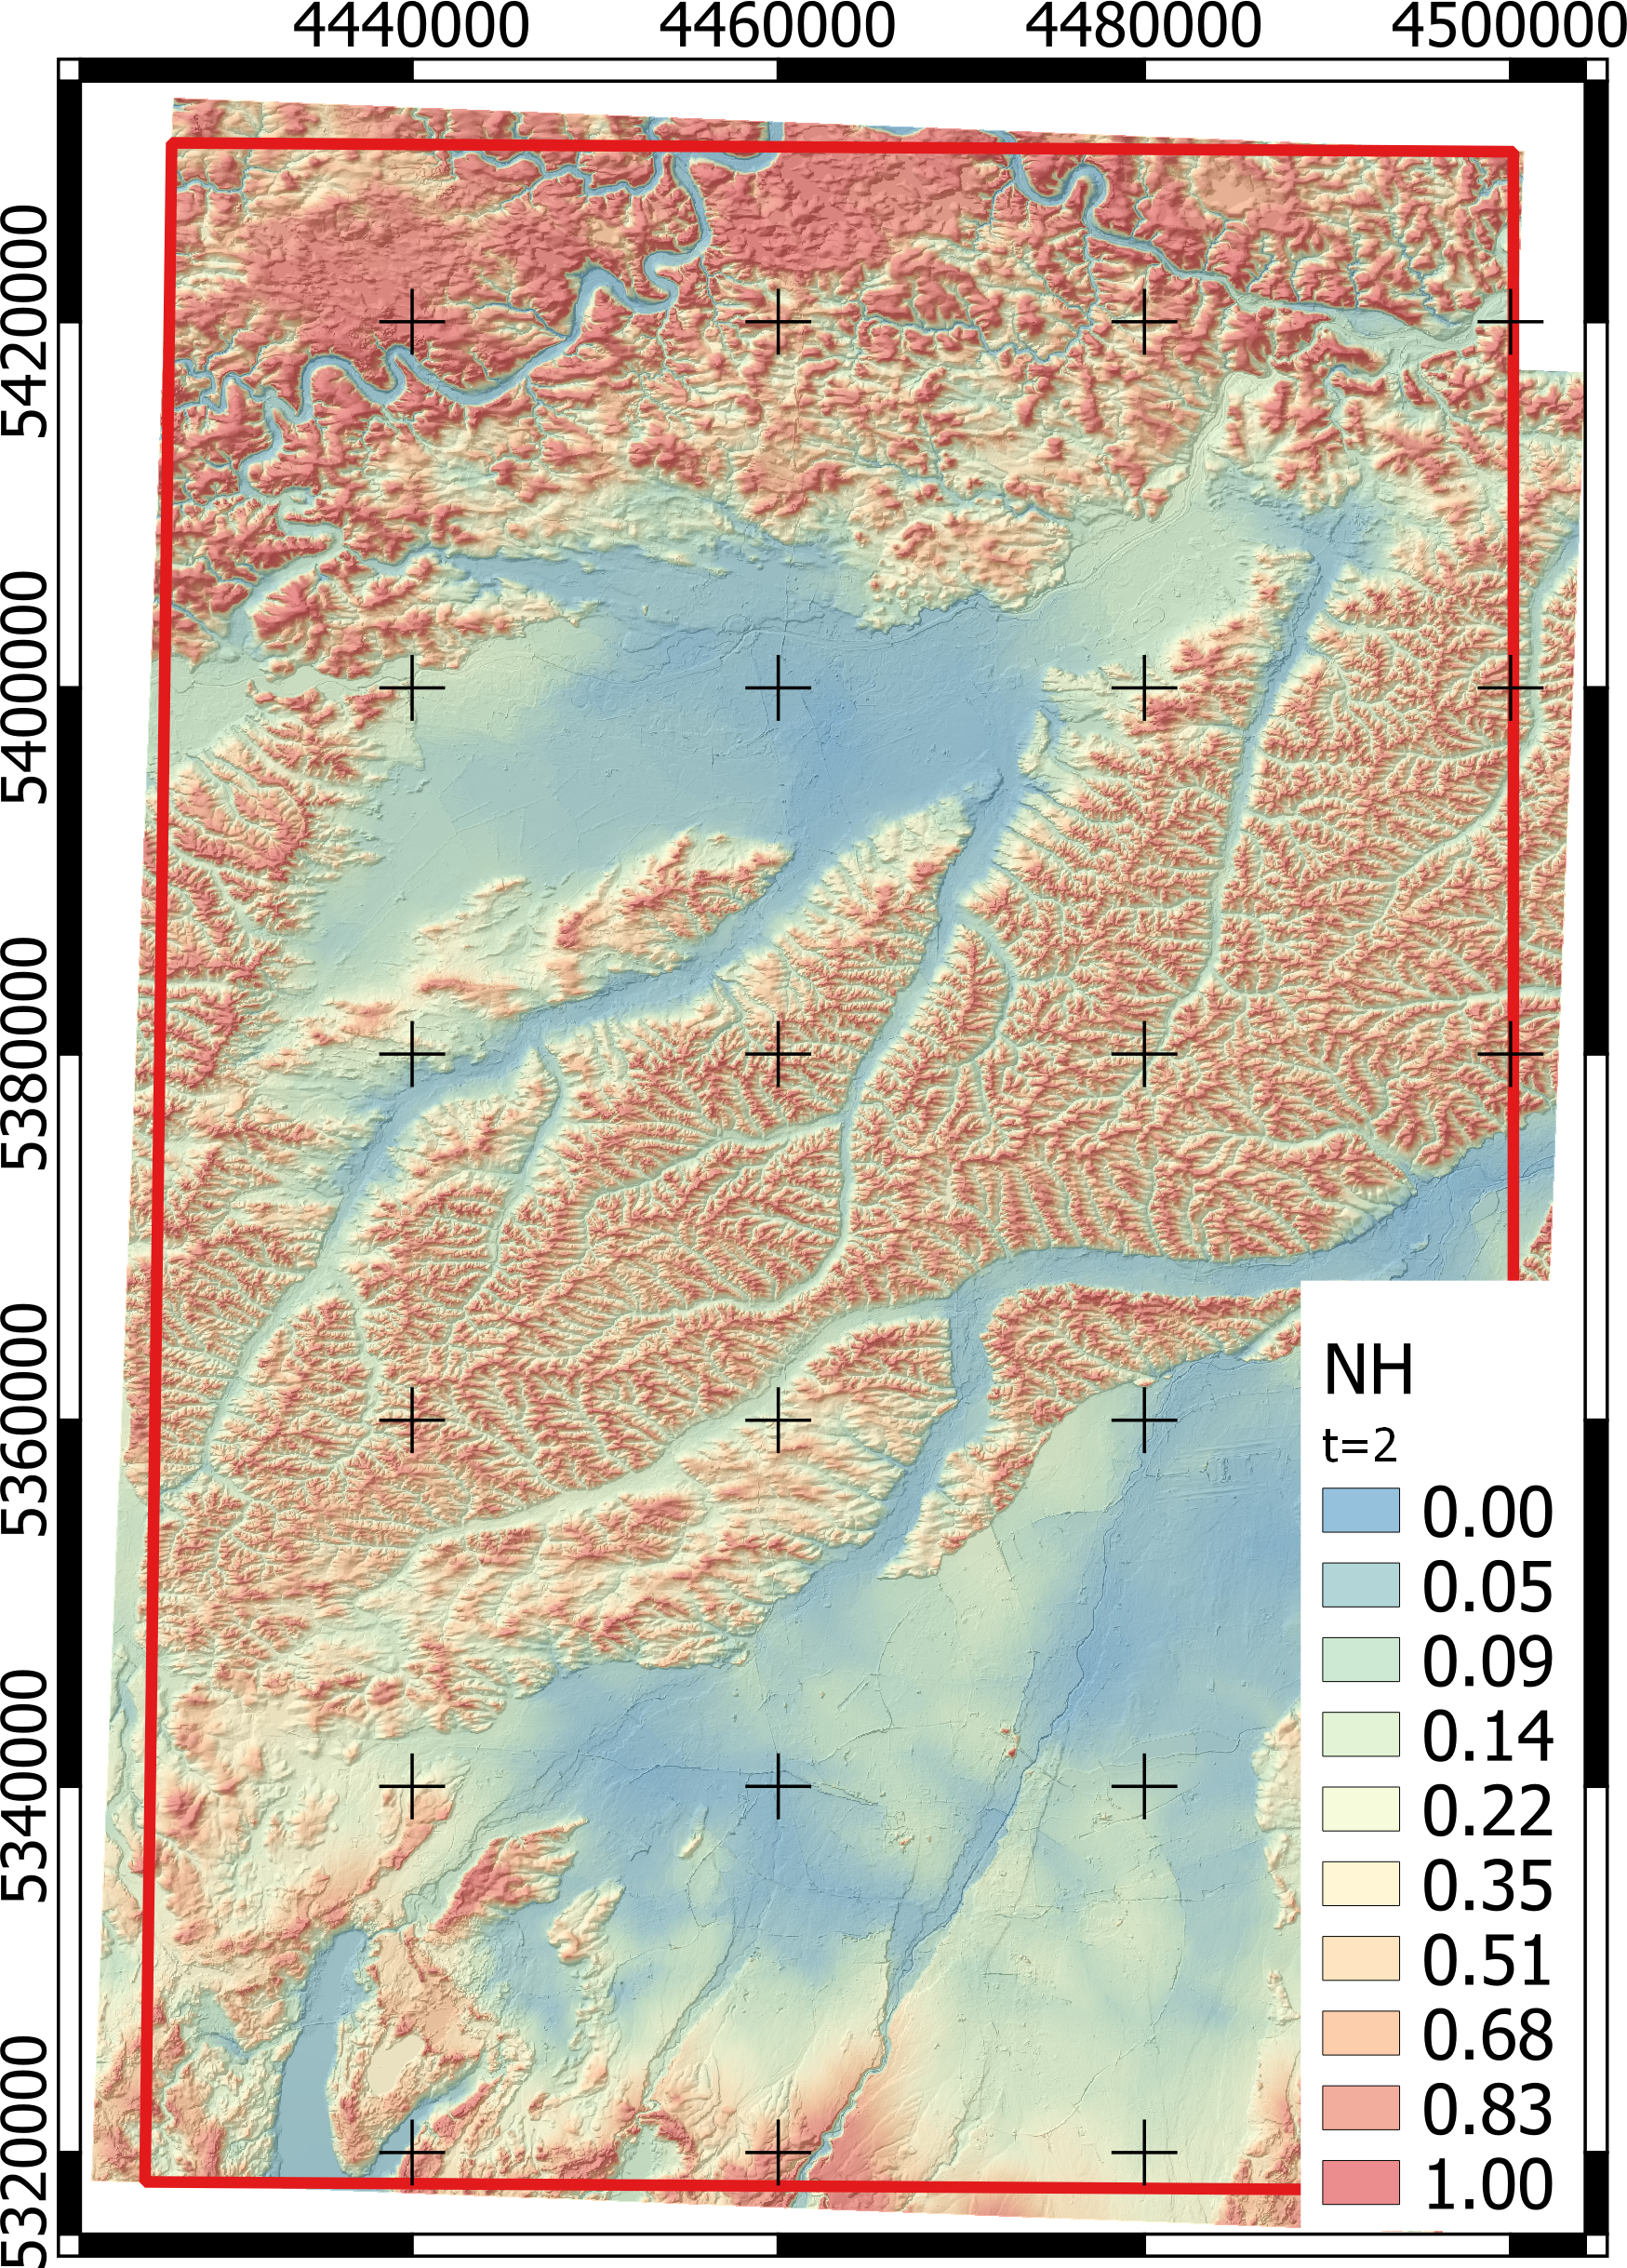
\includegraphics[width=1\textwidth]{FIGURE/Figure_NH-t2.png}
\end{block}
 \column{7cm}
 \begin{block}{Multi-hierarchische Reliefattribute}
 \centering\includegraphics[width=1\textwidth]{FIGURE/Table_TerrainAttributes.pdf}
 \end{block}
  \end{columns}
\end{frame}

%%%%%%%%%%%%%%%%%%%%%%%%%%%%%%%%%%%%%%%%%%%%%%%%%%%%%%%%%%%%%%%%%%%%%%%%%%%%%%%%%%%%%%%

\begin{frame}{Erklärende Variablen}
\begin{columns}
 \column{4cm}
 \begin{block}{$NH_{t=1000}$}
 \centering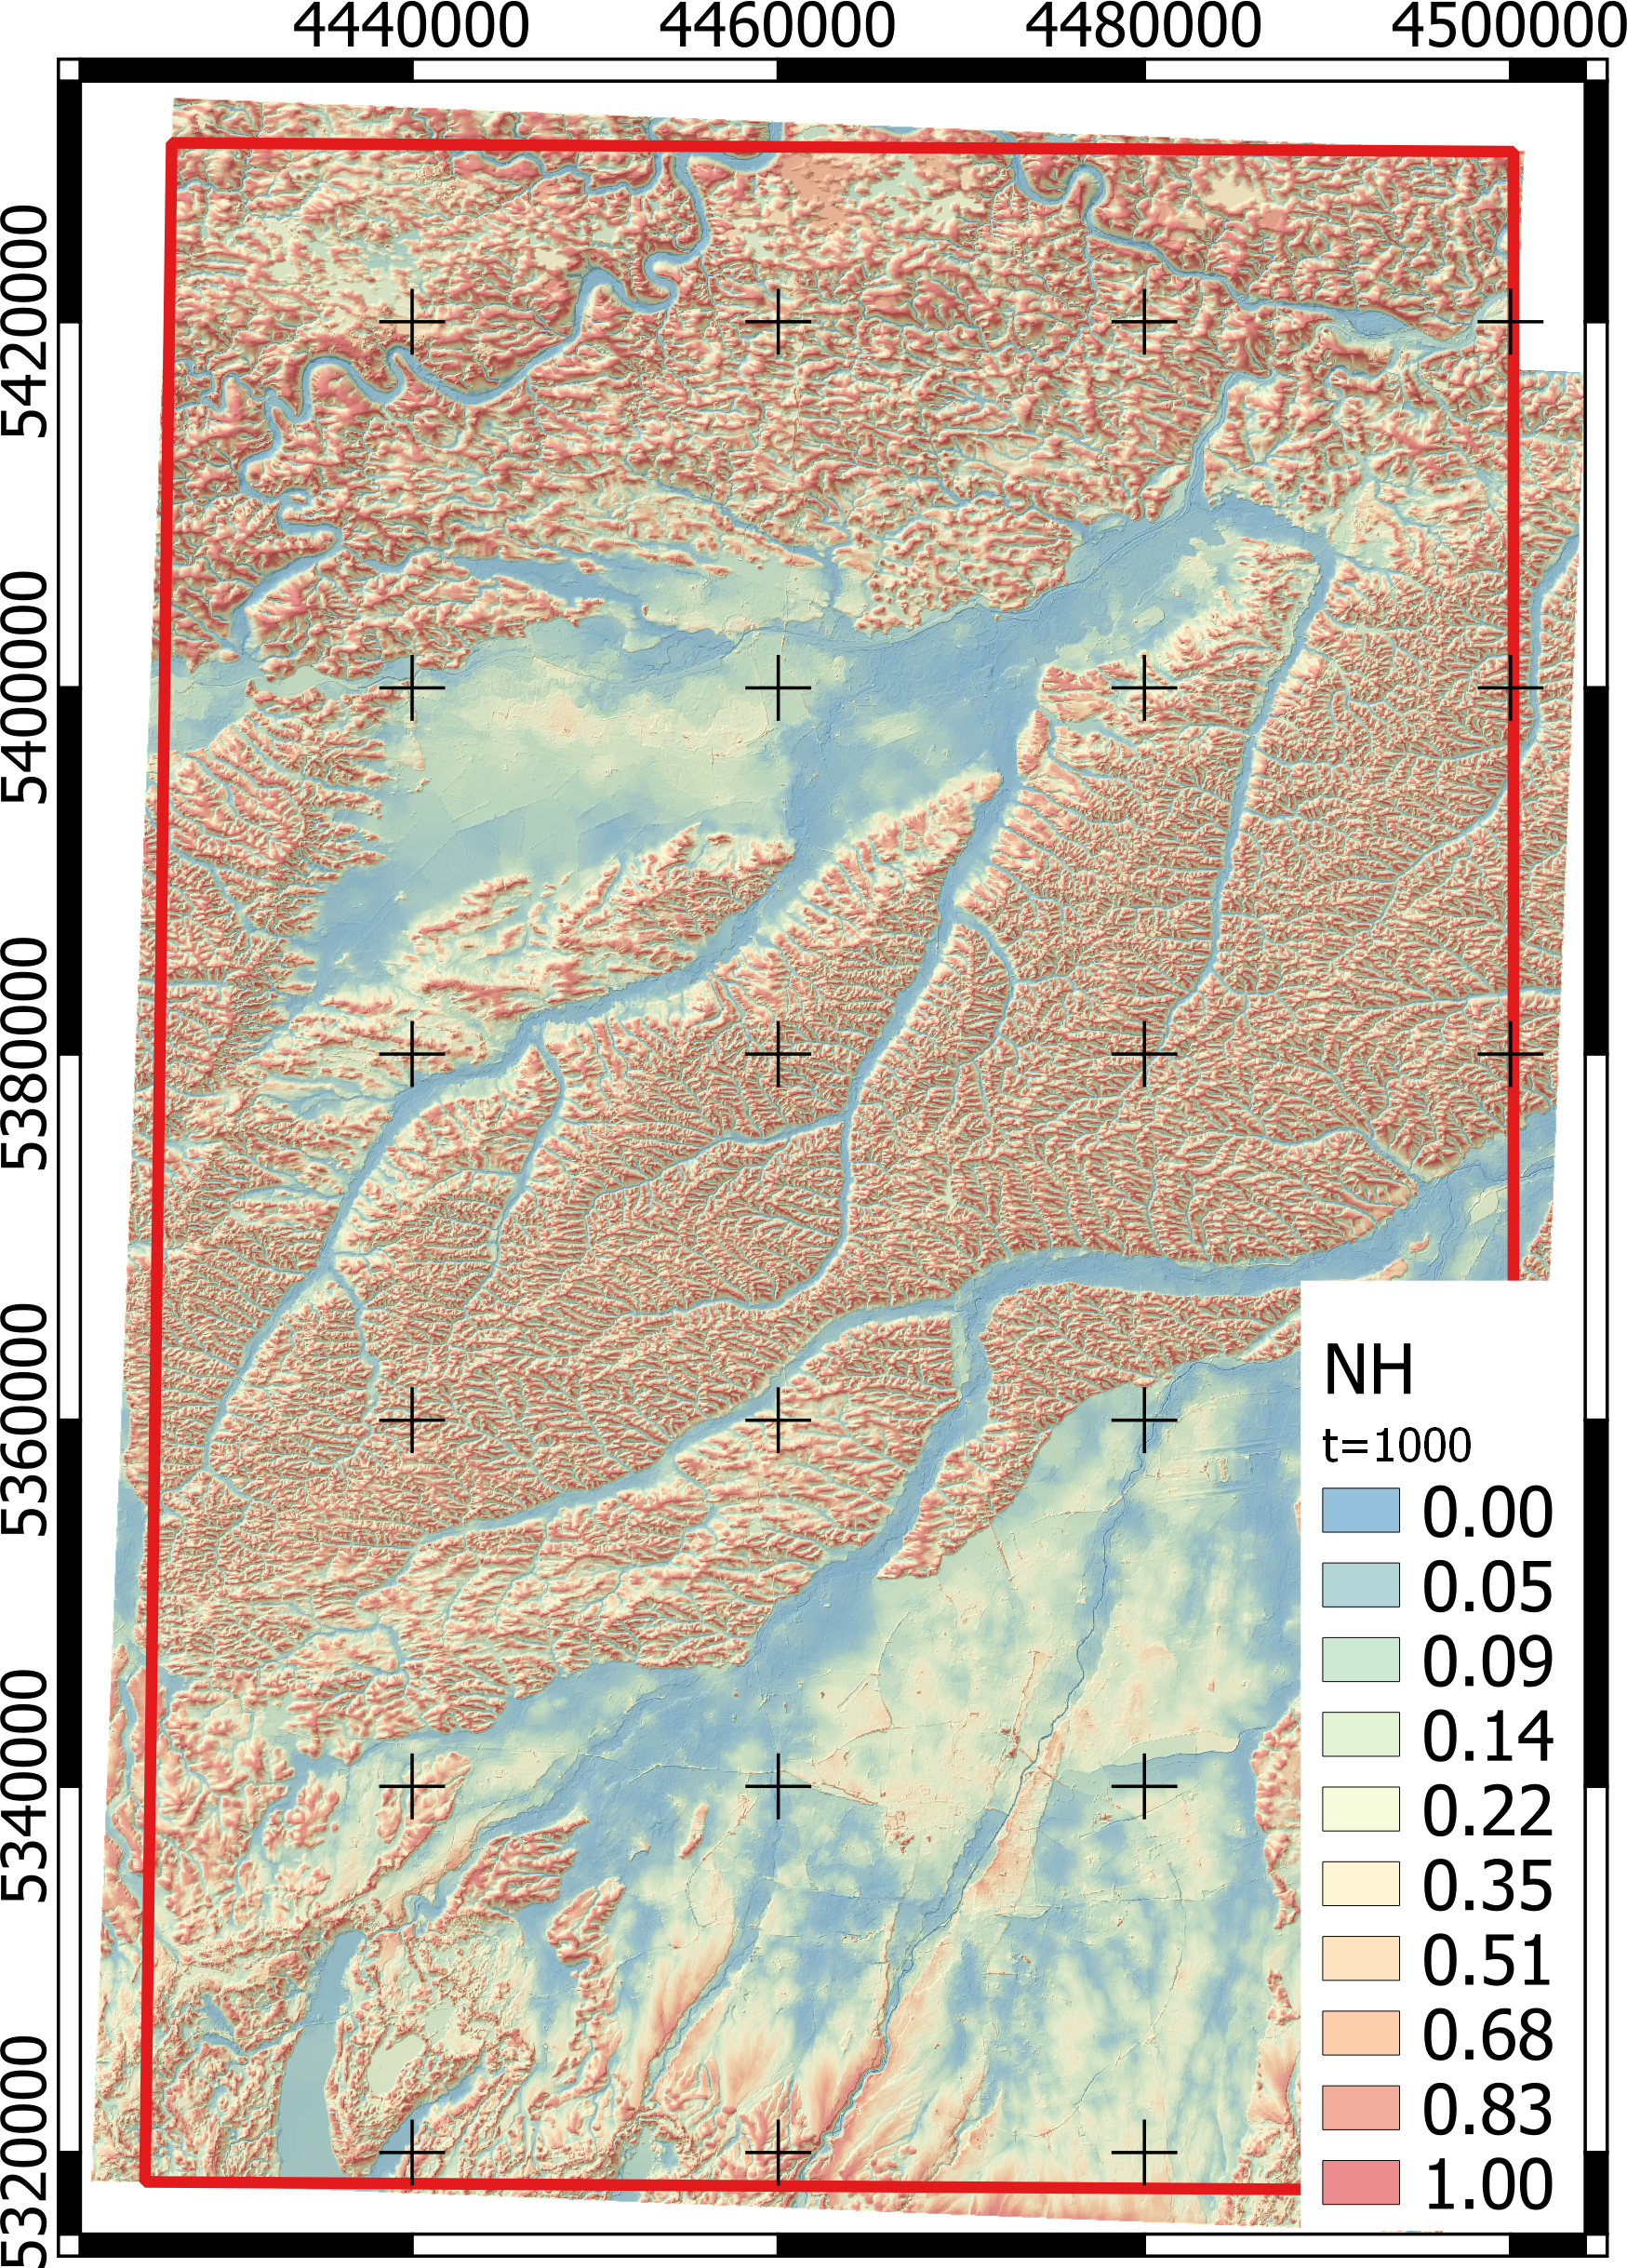
\includegraphics[width=1\textwidth]{FIGURE/Figure_NH-t1000.png}
\end{block}
 \column{7cm}
 \begin{block}{Multi-hierarchische Reliefattribute}
 \centering\includegraphics[width=1\textwidth]{FIGURE/Table_TerrainAttributes.pdf}
 \end{block}
% \raggedright\tiny 
%Möller, M., Zepp, S., Wiesmeier, M., Gerighausen, H., Heiden, U., 2022. Scale-Specific Prediction of Topsoil Organic Carbon Contents Using Terrain Attributes and SCMaP Soil Reflectance Composites. Remote Sensing 14, 2295. https://doi.org/10.3390/rs14102295          
  \end{columns}
\end{frame}

%%%%%%%%%%%%%%%%%%%%%%%%%%%%%%%%%%%%%%%%%%%%%%%%%%%%%%%%%%%%%%%%%%%%%%%%%%%%%%%%%%%%%%%

\begin{frame}{Multi-hierarchische Reliefobjekte}
\begin{columns}
 \column{6cm}
 \begin{block}{}
 \centering\includegraphics[width=1\textwidth]{FIGURE/Figure_Segmentation1.png}
\end{block}
 \column{5cm}
 \begin{block}{}
 \centering\includegraphics[width=1\textwidth]{FIGURE/Figure_Segmentation2.png}
 \end{block}
  \end{columns}
\raggedright\tiny 
\vspace{4,9pt}
 \begin{itemize}
     \item Möller M, Koschitzki T, Hartmann K-J, Jahn R. Plausibility test of conceptual soil maps using relief parameters. CATENA 2012;88:57–67. https://doi.org/10.1016/j  .catena.2011.08.002 .
     \item  Möller M, Volk M. Effective map scales for soil transport processes and related process domains — Statistical and spatial characterization of their scale-specific inaccuracies. Geoderma 2015;247–248:151–60. https://doi.org/10.1016/j  .geoderma.2015.02.003 .
%     \item  Möller M, Volk M, Friedrich K, Lymburner L. Placing soil-genesis and transport processes into a landscape context: A multiscale terrain-analysis approach. J Plant Nutr Soil Sci 2008;171:419–30. https://doi.org/10.1002/jpln.200625039  .
 \end{itemize}
\end{frame}

%%%%%%%%%%%%%%%%%%%%%%%%%%%%%%%%%%%%%%%%%%%%%%%%%%%%%%%%%%%%%%%%%%%%%%%%%%%%%%%%%%%%%%%

\begin{frame}{Erklärkraft}
\begin{columns}
\column{5.5cm}
\begin{block}{Zepp et al. (2021)}
\centering\includegraphics[width=1\textwidth]{FIGURE/Figure_Model_Accuracy-testsite.pdf}
\end{block}
\column{5.5cm}
\begin{block}{\alert{TA} ($L=6$)}
\centering\includegraphics[width=1\textwidth]{FIGURE/Figure_Model_Accuracy_TA_L6.pdf}
\end{block}
\end{columns}
\end{frame}

%%%%%%%%%%%%%%%%%%%%%%%%%%%%%%%%%%%%%%%%%%%%%%%%%%%%%%%%%%%%%%%%%%%%%%%%%%%%%%%%%%%%%%%

\begin{frame}{Erklärkraft}
\begin{columns}
\column{5.5cm}
\begin{block}{Zepp et al. (2021)}
\centering\includegraphics[width=1\textwidth]{FIGURE/Figure_Model_Accuracy-testsite.pdf}
\end{block}
\column{5.5cm}
\begin{block}{\alert{SCMaP-SRC} ($L=0.6$)}
\centering\includegraphics[width=1\textwidth]{FIGURE/Figure_Model_Accuracy_SM_L06.pdf}
\end{block}
\end{columns}
\end{frame}

%%%%%%%%%%%%%%%%%%%%%%%%%%%%%%%%%%%%%%%%%%%%%%%%%%%%%%%%%%%%%%%%%%%%%%%%%%%%%%%%%%%%%%%

\begin{frame}{Erklärkraft}
\begin{columns}
\column{5.5cm}
\centering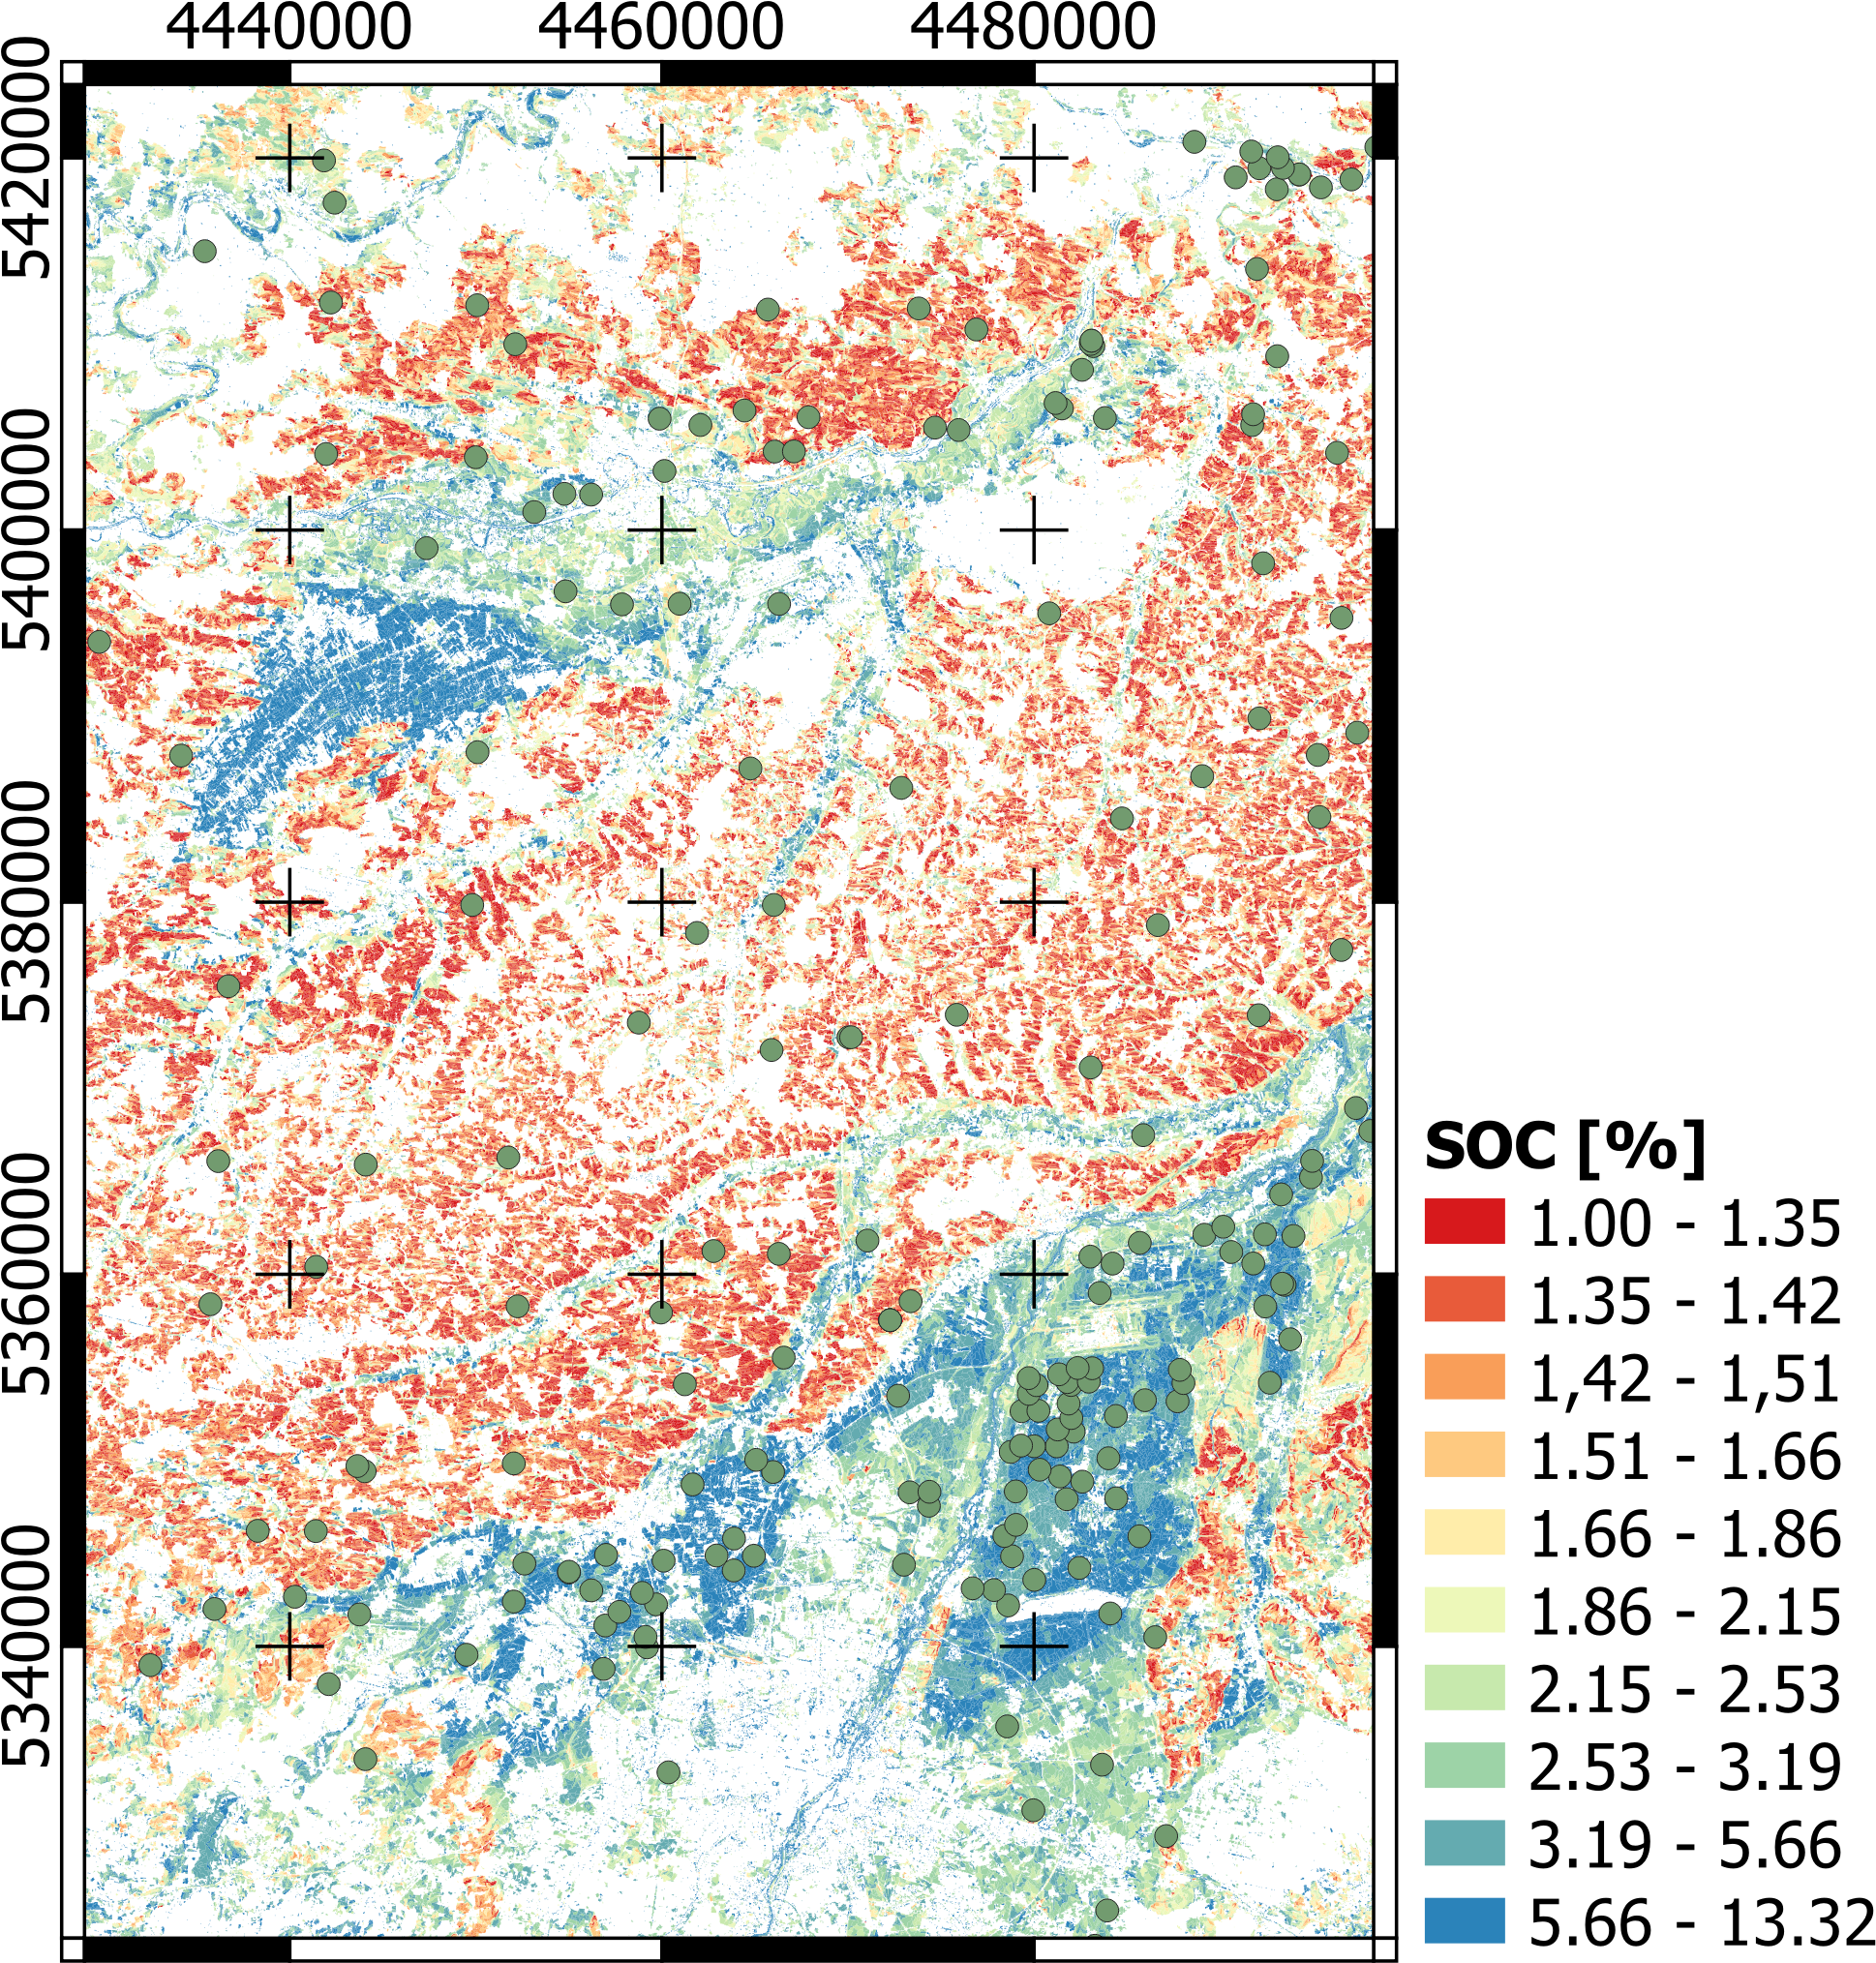
\includegraphics[width=1\textwidth]{FIGURE/Figure_SOC-content.png}

\column{5.5cm}
\begin{block}{\alert{TA+SCMaP-SRC} ($L=0.6$)}
\centering\includegraphics[width=1\textwidth]{FIGURE/Figure_Model_Accuracy_TA-SM_L06.pdf}
\end{block}
\end{columns}
\end{frame}

%%%%%%%%%%%%%%%%%%%%%%%%%%%%%%%%%%%%%%%%%%%%%%%%%%%%%%%%%%%%%%%%%%%%%%%%%%%%%%%%%%%%%%%

\begin{frame}{Erklärkraft}
\begin{columns}
\column{5.5cm}
\begin{block}{$R^2$}
\centering\includegraphics[width=1\textwidth]{FIGURE/Figure_R2.pdf}
\end{block}
\column{5.5cm}
\begin{block}{$RMSE$}
\centering\includegraphics[width=1\textwidth]{FIGURE/Figure_RMSE.pdf}
\end{block}
\end{columns}
\end{frame}

%%%%%%%%%%%%%%%%%%%%%%%%%%%%%%%%%%%%%%%%%%%%%%%%%%%%%%%%%%%%%%%%%%%%%%%%%%%%%%%%%%%%%%%

%\begin{frame}{Ergebnisse}
%\begin{block}{Regionale Prognose}
%\begin{columns}
%\column{5.7cm}
%\centering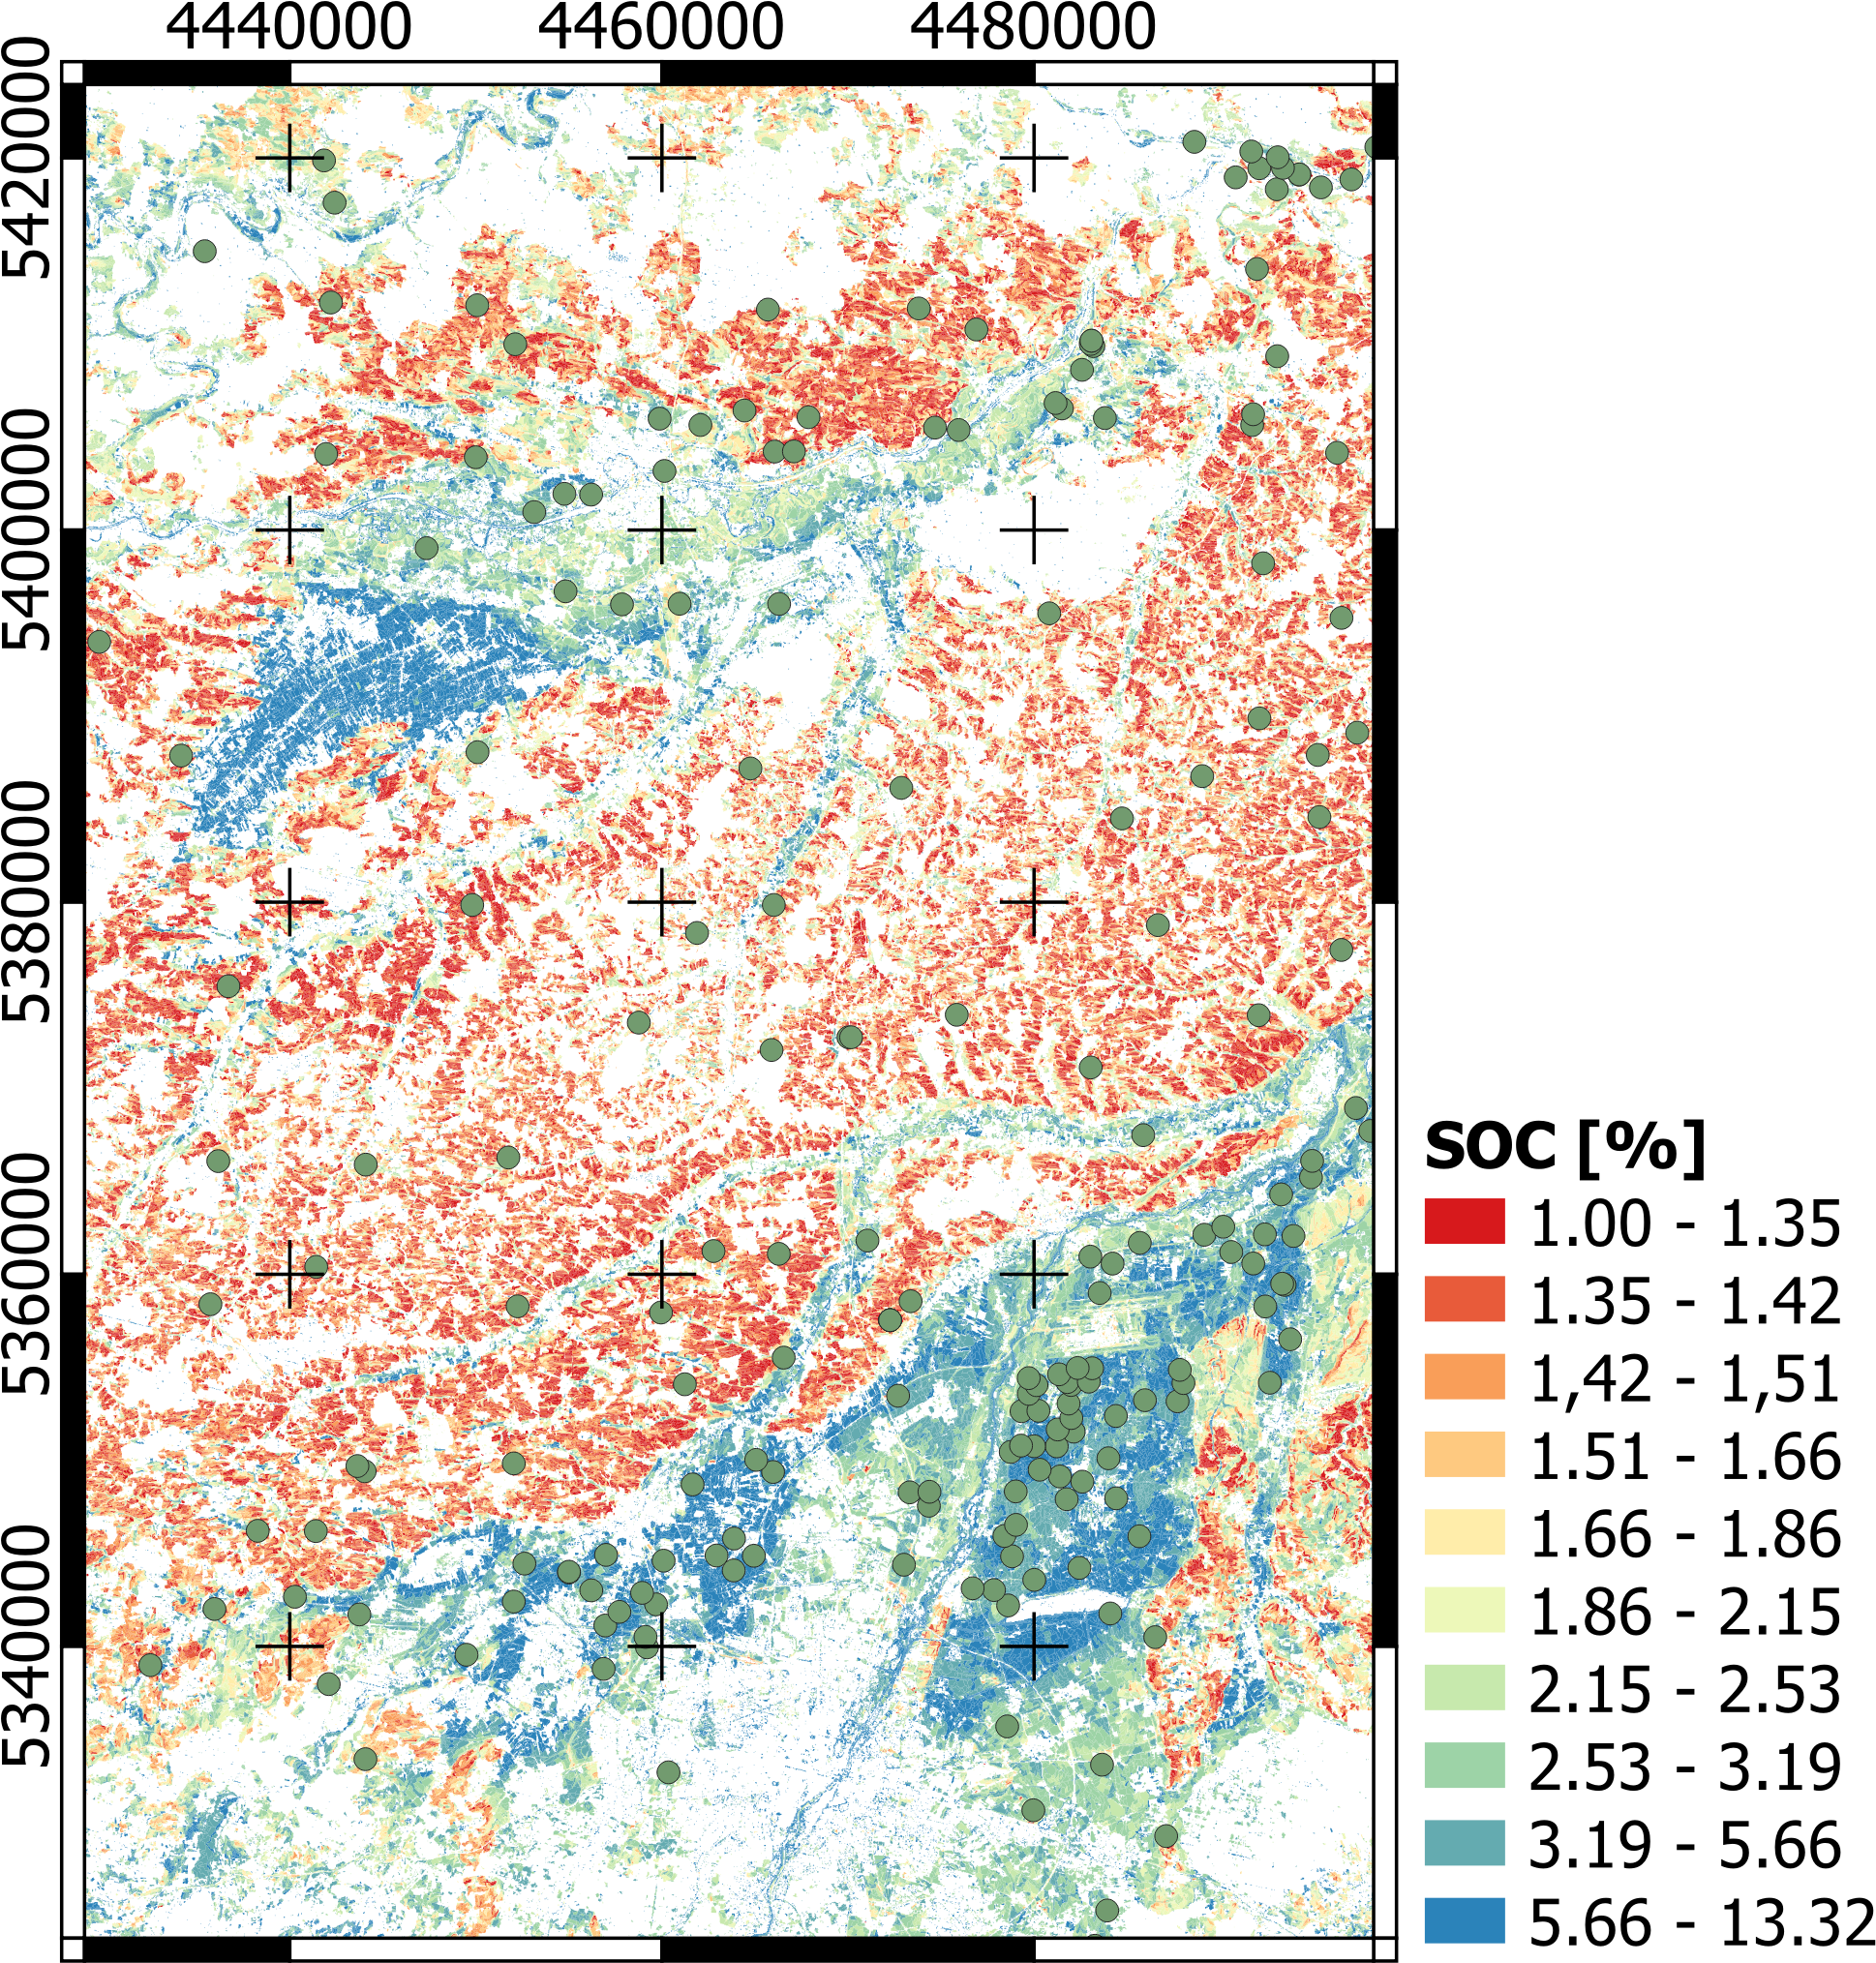
\includegraphics[width=1\textwidth]{FIGURE/Figure_SOC-content.png}

%\column{4.5cm}
%\alert{\footnotesize SCMaP-SCMaP-SRC}
%\centering\includegraphics[width=0.7\textwidth]{FIGURE/Figure_Model_Accuracy-testsite.pdf} 

%\alert{\footnotesize SCMaP-SRC +  TA}
%\centering\includegraphics[width=0.7\textwidth]{FIGURE/Figure_Model_Accuracy_TA-SM_L06.pdf}
%\end{columns}
%\end{block}

%\raggedright\tiny \href{https://doi.org/10.3390/rs14102295}{Möller,         M., Zepp, S., Wiesmeier, M., Gerighausen, H., Heiden, U., 2022. Scale-Specific Prediction of Topsoil Organic Carbon Contents Using Terrain Attributes and SCMaP Soil Reflectance Composites. Remote Sensing 14, 2295.} 
%\end{frame}



%\begin{frame}{Ergebnisse}
%\begin{block}{Code}
% \centering\includegraphics[width=1\textwidth]{FIGURE/ScaleP1.png} 
%\end{block}    
%\begin{tabular}{ll}
%\centering\includegraphics[width=0.07\textwidth]{FIGURE/Octocat.png} &
%\centering\includegraphics[width=0.5\textwidth]{FIGURE/Zenodo.png}\\
%\end{tabular}
%\end{frame}


\begin{frame}{Zusammenfassung}
\begin{alertblock}{Maßstabsspezifische Optimierungen können die Güte von SOC-Prognosemodellen verbessern.}
\begin{itemize}
\item Es gibt Abhängigkeiten zwischen der maßstabsspezifischen Repräsentativität der Bodenproben und der Erklärungskraft der verwendeten Variablen. 
\item Im Vergleich zu Reliefattributen zeichnen sich Parameter, die auf multi-temporalen Bodenreflexionskompositen basieren, durch eine höhere Erklärungskraft auf großen Maßstäben aus. 
\item Die Erklärungskraft von Reliefattributen ist im Allgemeinen geringer, aber über die Skalenebenen hinweg ausgewogener.
\end{itemize}
\end{alertblock}   


\end{frame}

\begin{frame}{Ausblick}

\begin{block}{Deutschlandweite raum-zeitliche Modellierung von \textcolor{red}{Ko}hlenstoffgehalten
landwirtschaftlicher \textcolor{red}{Bö}den durch eine integrative Auswertung von
\textcolor{red}{S}atellitenbildzeitreihen und Geodaten (\textcolor{red}{KoBoS})}
\textbf{Regionale maßstabsspezifische Prognosekarten des Kohlenstoffgehaltes landwirtschaftlicher Böden mit Genauigkeitsmetriken}
\begin{itemize}
    \item Bereitstellung von Webdiensten deutschlandweit erklärender erklärenden Variablen nach FAIR-Prinzipien,
    \item Entwicklung eines erweiterbaren, dynamischen und webbasierten Open-Source-Modells, das für beliebige Gebiete in Deutschland anwendbar ist.
    \end{itemize}
\end{block}

\footnotesize gefördert durch das BMEL-Klimaschutz-Sofortprogramm 2022 \newline\#RessortForschtKlima

\end{frame}



\begin{frame}{\alert{Fragen?}}
 \centering\includegraphics[width=1\textwidth]{FIGURE/big_cover-remotesensing-v14-i10.png}     
\end{frame}

\end{document}


